% Downloaded from http://www.dfcd.net/articles/latex/latex.html
% Modified by CC He.
% Notes on how to use this header is on Dropbox/Latex_Templates/LaTeX_for_Physicists/README.md
% ***********************************************************
% ******************* PHYSICS HEADER ************************
% ***********************************************************
% Version 2

\documentclass[12pt]{article}
\usepackage{setspace}
\usepackage{amsmath} % AMS Math Package
%\usepackage{fontspec,unicode-math}
%\usepackage{amsthm} % Theorem Formatting
\usepackage{amssymb}	% Math symbols such as \mathbb
\usepackage{units}
\usepackage{listings}
\usepackage{hyperref}
\usepackage{graphicx} % Allows for eps images
\usepackage{multicol} % Allows for multiple columns
\usepackage[dvips,letterpaper,margin=0.75in,bottom=0.5in]{geometry}
\usepackage{natbib}
\usepackage{float}

% Define ads acronyms
\newcommand{\apj}{ApJ}
\newcommand{\apjl}{ApJL}
\newcommand{\apjs}{ApJS}
\newcommand{\aap}{A\&A}
\newcommand{\araa}{ARA\&A}
\newcommand{\ssr}{SSR}
\newcommand{\mnras}{MNRAS}


 % Sets margins and page size
\pagestyle{empty} % Removes page numbers
%\pagestyle{fancy}
\makeatletter % Need for anything that contains an @ command 

\newcommand{\code}{\lstinline}
\renewcommand{\tt}{\texttt}
\newcommand{\m}{\textrm}
\renewcommand{\maketitle} % Redefine maketitle to conserve space
{ \begingroup \vskip 10pt \begin{center} \large {\bf \@title}
	\vskip 10pt \large \@author \hskip 20pt \@date \end{center}
  \vskip 10pt \endgroup \setcounter{footnote}{0} }
\makeatother % End of region containing @ commands
\renewcommand{\labelenumi}{(\alph{enumi})} % Use letters for enumerate
% \DeclareMathOperator{\Sample}{Sample}
\let\vaccent=\v % rename builtin command \v{} to \vaccent{}
\renewcommand{\v}[1]{\ensuremath{\mathbf{#1}}} % for vectors
\newcommand{\gv}[1]{\ensuremath{\mbox{\boldmath$ #1 $}}} 
% for vectors of Greek letters
\newcommand{\uv}[1]{\ensuremath{\mathbf{\hat{#1}}}} % for unit vector
\newcommand{\abs}[1]{\left| #1 \right|} % for absolute value
\newcommand{\avg}[1]{\left< #1 \right>} % for average
%\let\underdot=\d % rename builtin command \d{} to \underdot{}
\renewcommand{\d}[1]{\mathrm{d}#1} % for differential
\newcommand{\dd}[2]{\frac{\d{#1}}{\d{#2}}} % for derivatives
\newcommand{\ddd}[2]{\frac{\mathrm{d}^2 #1}{\d{#2^2}}} % for double 
%derivatives
\newcommand{\pd}[2]{\frac{\partial #1}{\partial #2}} 
% for partial derivatives
\newcommand{\pdd}[2]{\frac{\partial^2 #1}{\partial #2^2}} 
% for double partial derivatives
\newcommand{\pdc}[3]{\left( \frac{\partial #1}{\partial #2}
 \right)_{#3}} % for thermodynamic partial derivatives
\newcommand{\ket}[1]{\left| #1 \right>} % for Dirac bras
\newcommand{\bra}[1]{\left< #1 \right|} % for Dirac kets
\newcommand{\braket}[2]{\left< #1 \vphantom{#2} \right|
 \left. #2 \vphantom{#1} \right>} % for Dirac brackets
\newcommand{\matrixel}[3]{\left< #1 \vphantom{#2#3} \right|
 #2 \left| #3 \vphantom{#1#2} \right>} % for Dirac matrix elements
\newcommand{\grad}[1]{\gv{\nabla} #1} % for gradient
\let\divsymb=\div % rename builtin command \div to \divsymb
\renewcommand{\div}[1]{\gv{\nabla} \cdot #1} % for divergence
\newcommand{\curl}[1]{\gv{\nabla} \times #1} % for curl
\let\baraccent=\= % rename builtin command \= to \baraccent
\renewcommand{\=}[1]{\stackrel{#1}{=}} % for putting numbers above =
\newtheorem{prop}{Proposition}
\newtheorem{thm}{Theorem}[section]
\newtheorem{lem}[thm]{Lemma}
%\theoremstyle{definition}
\newtheorem{dfn}{Definition}
%\theoremstyle{remark}
%\newtheorem*{rmk}{Remark}


% Define \stretchint, a macro to input large integrals.
\usepackage{scalerel}[2016-12-29]
\def\stretchint#1{\vcenter{\hbox{\stretchto[440]{\displaystyle\int}{#1}}}}
\def\scaleint#1{\vcenter{\hbox{\scaleto[3ex]{\displaystyle\int}{#1}}}}
\def\bs{\mkern-12mu}

\usepackage{graphicx}
\usepackage{subcaption}

\begin{document}

\title{ASTR615 HW\#4}
\author{Group 4: ChongChong He \& }
\date{\today}
\maketitle

\section*{Problem 2}
We perform a series of simulations of globular clusters.

\subsection*{Stellar Cluster}
%\subsubsection*{Setups}
We did a few simulations of stellar clusters with made-up initial conditions 

\subsubsection*{Mass distribution}
We implement in all of our simulations the Kroupa IMF:
\begin{equation}
\phi(m) \propto 
\begin{cases}
m^{-1.3} \; &(0.08M_\odot < m < 0.5M_\odot) \\
0.5 \, m^{-2.3} \; &(0.5M_\odot<m<100M_\odot)
\end{cases}
\end{equation}
after doing transformation we get
\begin{equation}
m=
	\begin{cases}
	-\cfrac{0.566179}{\sqrt[3]{1.7987\, - x} \left(x^3-5.39611 
	x^2+9.70599 x-5.81939\right)} & (0<x<0.760707) \\
	\cfrac{0.166558}{(1.00024\, -x)^{10/13}} & (0.760707<x<1)
	\end{cases}
\end{equation}
where $ x $ is a random number between 0 and 1. Figure \ref{fig:imf} shows the 
histogram of the masses of the generated particles as compared to the analytical line.
\begin{figure}[h]
	\centering
	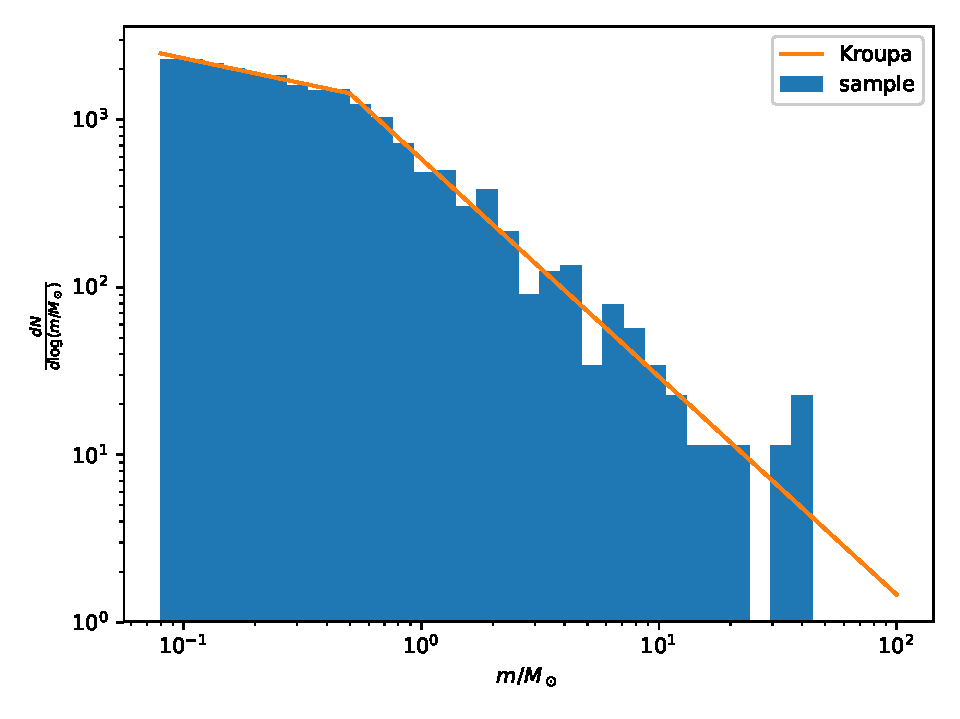
\includegraphics[width=.6\columnwidth]{../simulations/imf.pdf}
	\caption{The mass distribution of the particles in our simulation compared to analytical 
	Kroupa IMF lines.}
	\label{fig:imf}
\end{figure}

\subsubsection*{Spacial and velocity distribution}
The cluster is a specially uniformly distributed sphere with a radius of 1. The initial 
velocities are from a  Gaussian distribution with a dispersion correspondent to a virial ratio 
of $ \alpha \sim 0.4 $. A virial ratio $ \alpha < 0.5 $ implies the system is bounded. The 
velocity dispersion in one axis is $ \sigma_x = 11.4 $ and the crossing time is $ t \approx 
0.08 $, so we use a step size of 0.0005, i.e. 160 steps per crossing time.

\subsubsection*{Softening parameter and step size}
However, the binary radius is $ \sim 10^{-3} $ and the period is of order $ 10^{-4} $, so our 
resolution it is far away from resolving binary particles. In order to avoid binaries, we use 
a large softening parameter $ \epsilon = 0.005 $. We also do a control run with $ \epsilon 
= 10^{-5} $ to be compared with (Figure \ref{fig:energy}).

\subsubsection*{Results: Energy and Time Consumption}
The total number of particles in our simulation is 1000. We run this simulation with both 
our PP-nbody code and BH-nbody code. The energy curve through 400 steps is shown in 
Figure \ref{fig:energy}. When the softening parameter is too small, the energy of the 
system increases dramatically due to close encounters being threw away with large step 
sizes. 

As for PP-nbody vs. BH-nbody, in our simulations of 1000 particles, BH code has nearly 
no advantage. With a step size 0.0005 and softening parameter 0.005, when running for 
400 steps, i.e. 2 - 3 dynamic time, PP code conserves energy better then BH code, even 
with a small critical angle, and the BH code is not effective faster.
It takes 21.0 seconds for the PP code to run the simulation, 15.0 seconds for the BH code 
with theta = 0.6, and 31.8 seconds for the BH code with theta = 0.3.
%PP-nbody, time elapsed: 21.007760047912598
%BH-nbody, time elapsed: 15.026080846786499
%BH-nbody, time elapsed: 31.776031970977783
The videos are shown in \textit{simulations/} as \textit{cluster\_rotating\_camera.mp4} and 
\textit{cluster\_static\_camera.mp4}.
\begin{figure}
		\centering
	\begin{subfigure}[b]{0.48\textwidth}
		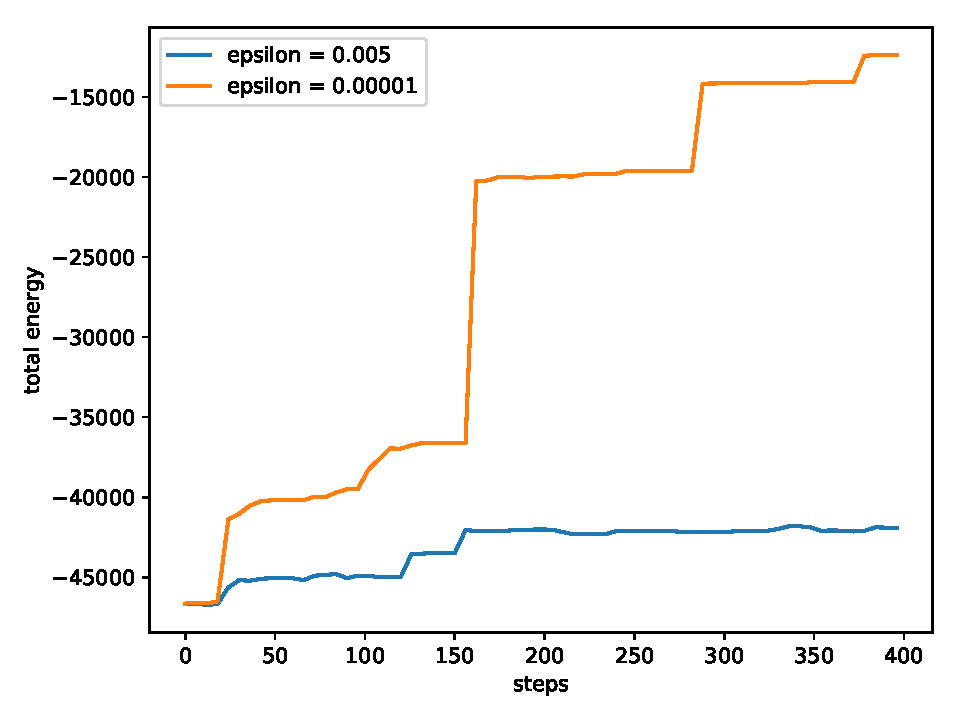
\includegraphics[width=\columnwidth]{../simulations/energy_compare_epsilon}
		\label{fig:energycompareepsilon}
	\end{subfigure}
	\begin{subfigure}[b]{0.48\textwidth}
		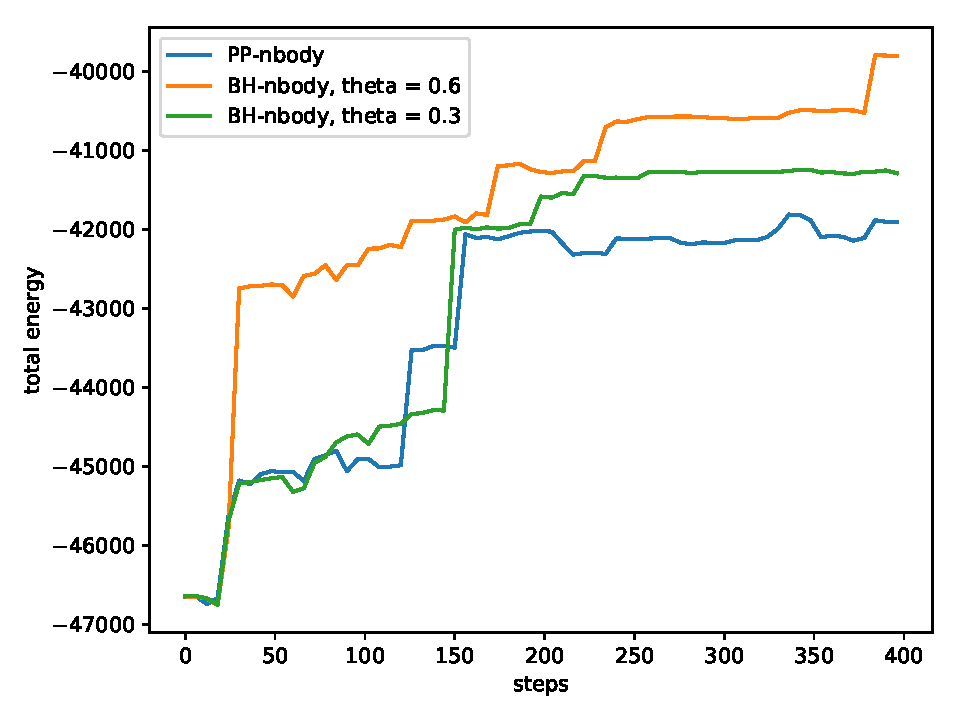
\includegraphics[width=\columnwidth]{../simulations/energy_compare_PP_BH}
		\label{fig:energycompareppbh}
	\end{subfigure}
	\caption{Energy curve of the systems in our simulations of stellar clusters. All 
	simulations use the same initial conditions but different softening parameters (left) 
	and different methods of force calculation, i.e PP vs BH-tree (right). Epsilon is the 
	softening parameter and theta is the critical angle in BH-tree. In the simulations shown 
	in the right panel, epsilon = 0.005.}
	\label{fig:energy}
\end{figure}

%\subsubsection*{Energy conservation and step sizes}

%\subsection*{Binary Problem}
\subsection*{RAMSES-RT}
We also use initial conditions taken from a snapshot of a simulation from 
\textit{RAMSES-RT}, an AMR MHD code with radiative transfer. A total of 820 particles are 
formed from a cold molecular cloud. This work is not shown in the directory due to limited 
time, but I use the units and time scales in this simulation to investigate into binary 
problem. 

\subsubsection*{Units and Time Scales}
The units in this simulation are as follow: $ [T] = 2.5395 \times 10^{15}\,$s $\approx 
80\,$Myr, $ [L] = 3.08 \times 10^{18} \, $cm $ \approx 1 \, $pc, $ [M] = 6.7925 \times 
10^{31} \, $g $ \approx 0.03416 M_\odot $. In this setup the gravitational constant is unity. 

Imaging a cluster of stars from the outputs of \textit{RAMSES} simulation which has $ \sim 
$ 1000 stars with Kroupa IMF located in a box of length $ L = 50 $. If this system is 
virialized, then $ \sigma^2 = M_{\rm tot} / R $, from which we obtain $ \sigma \approx 
27 $. Here I use a mean mass of 0.638 $ M_\odot $ = 20 (code unit) from Salpeter IMF and 
$ R = 25 $.
Then, the crossing time of dispersion velocity is $ t_{\sigma} = L / \sigma \approx 2 $.
If we choose a step size $ \Delta t  = t_\sigma / 50 = 0.04 $, i.e. 50 steps in a crossing time, 
then with 5000 steps we are able to simulate 100 crossing time, which is equal to 16 Gyr. 
This can be done with a PP n-body code on my laptop, and it could be even faster with our 
BH-tree n-body code.

\subsection*{Binary Problem}
I have an attempt on solving the problem of binarity in stellar cluster simulation.
The basic idea is to check if two particles 1) are close enough to each other, and 2) $ K + V 
< 0 $ every $ n $ steps. If yes, we just replace these two particles with one star 
representing the motion of the center of mass. Binaries may further merge into trinaries 
and so on.

\subsubsection*{Realization of the Binary Problem}
If two stars with velocities $ \sigma $ are in virial equilibrium, i.e. $ \alpha = K/|W| = 0.5 
$, the separation between them would be $ d_{\rm virial} = m /2 \sigma^2 = 0.016 $. 
However, the typical displacement of a particle in one step is $ d_{\rm step} = \sigma \Delta 
t \approx 1 $, much greater than $ d_{\rm virial} $. Therefore our simulation is not able to 
identify binary stars. We need a step size $ \sim $1000 times smaller to achieve the 
resolution of binary systems.

\subsubsection*{Searching for close encounters}
We consider two stars in the center-of-mass frame. We defined the following two 
parameters:
\begin{itemize}
	\item The \textit{close-encounter parameter} $ \alpha $ or $ \gamma $ which defines the 
	criteria of being close enough to each other:
	\begin{equation}\label{eq:r12}
	| \v{r}_1 - \v{r}_2 | < d_{\rm close} = \alpha \cdot d_{\rm virial} = \gamma \cdot d_{\rm step}.
	\end{equation}
%	where $ \alpha $ is a parameter to be determined.
	\item The \textit{escape parameter} $ \beta $ which confines the particles in a small 
	region:
	\begin{equation}\label{key}
	\frac{K}{|W|} < 1 - \beta^{-1}.
	\end{equation}
	This relation gives the largest separation between the two particles at any time, 
	\begin{equation}
	d_{\rm max} = \beta d_{\rm close},
	\end{equation}
	ignoring interactions with other particles
	\footnote{This relation is obtained by solving  equation $ (1 - \beta^{-1}) |V_0| + V_0 = 0 
	+ V_1 $ and $ V_0 \propto 1/d_0 $,	$ V_1 \propto 1/d_{\rm max} $.}.
	When $ d_{\rm max} \ll d_{\rm step} $ the two particles may be considered as a 
	binary.
\end{itemize}

The solution to binary problem then becomes the balancing between typical particle 
separation $ d_{\rm sepa} = L/\sqrt[3]{N} $, one-step displacement $ d_{\rm 
step} = \sigma \Delta t $, the close-encounter parameter $ \alpha $ or $ \gamma $, and 
the escape parameter $ \beta $.

\subsection*{Results}
To test our code, we artificially create a three-body system and show that a binary system 
will appear when the step size is small enough. However, it will not be resolved when 
running with large step sizes. When we implement our BH-nbody Binary code, it 
successfully catches the binary when running with the same large step size. The movies 
of the three run described above are shown \textit{simulations/binary/movie}. We were 
working on this in a new branch. Due to limited amount of time we couldn't merge it to our 
master branch. We just show the videos here.

%With $ d_{\rm sepa} \sim 5 $, we set $ \Delta t = 0.04 $, $ \alpha = 5 $ and $ \beta = 2 $, 
%which imply $ d_{\rm step} = 1 $, $ d_{\rm close} = 0.08 $, and $ d_{\rm max} = 0.16 $.

%\begin{figure}
%	\centering
%	\caption{The tree code fails to resolve the binary system after a few orbits. Here $ 
%	\epsilon = 10^{-5}, \Delta t = 10^{-5}, 4000 steps per output. $}
%\end{figure}

%\subsection*{Morphology}
%We use disk galaxies in our simulation. Each disk galaxy has two components: a 
%thin disk and a thick disk. Each component has a density profile $ \rho(r, h) = 
%\rho_0 \, e^{-r/r_{\rm H}} \, e^{-h/h_{\rm H}} $. $ r $ and $ h $ are given by the 
%solution to the equation
%\begin{equation}\label{key}
%	x = 1 - (1 + \frac{r}{r_{\rm H}}) \, e^{-\frac{r}{r_{\rm H}}}
%\end{equation}
%where $ x $ is a uniform random number between 0 and 1.

%\subsection*{Disk Rotation}
%We use a uniform angular velocity $ \omega $.

%\subsection*{Setups}
%\begin{table}[h]
%	\centering
%	\begin{tabular}{ccccc}
%%		\hline{}
%		& $M/M_\odot$ & $r_{\rm H}$/kpc & $h_{\rm H} $/kpc & $\omega/?$ \\
%		\hline
%		thin disk & $5 \times 10^{10}$ & 3.5 & 0.3 & 1? \\
%		thick disk & $ 0.75 \times 10^{10} $ & 3.5 & 1.0 & 1? \\
%%		\hline
%	\end{tabular}
%	\caption{Parameters and errors from Lorentzian and Gaussian fits.}
%	\label{fit params}
%\end{table}
%
%\subsection{Units}
%[L] = kpc, [M] = $ 10^9 M_\odot $, [T] = 14.91 Myr.


\end{document}